\documentclass[12pt,thmsa]{article}

%maths
\usepackage{amsmath}   % \sideset
\usepackage{amsthm}    % for proof
\usepackage{amsfonts}  % for \mathbb
\usepackage{mathrsfs}  % for Ralph Smith's Formal Script Font
\usepackage[mathscr]{euscript} %redefine the \mathcal command to use Euler script
\usepackage{amssymb}   % \varnothing, \bigstar, \blacksquare, \clubsuit, \blacktriangleright, \diamondsuit, \spadesuit, \dagger, \checkmark

%algorithms
\usepackage{algorithm} % http://ctan.org/pkg/algorithms
\usepackage{algpseudocode}% http://ctan.org/pkg/algorithmicx

%tables
\usepackage{booktabs}  % Allows the use of \toprule, \midrule and \bottomrule in tables
\usepackage{multirow}
\usepackage{multicol}
\usepackage{tabularx}
\usepackage[table]{xcolor} % For \cellcolor
\usepackage[export]{adjustbox}

%figures
\usepackage{graphicx}  % Allows including images
\usepackage{float}     % Force figure placement in text with [H]

%tikzpicture
\usepackage{tikz}
\usepackage{scalerel}
\usepackage{pict2e}
\usepackage{tkz-euclide}
\usetikzlibrary{matrix}
\usetikzlibrary{shapes, positioning}
\usetikzlibrary{calc}
\usetikzlibrary{patterns, arrows.meta}
\usetikzlibrary{shadows}
\usetikzlibrary{external}

%pgfplots
\usepackage{pgfplots}
\pgfplotsset{compat=newest}
\usepgfplotslibrary{statistics}
\usepgfplotslibrary{fillbetween}

%colors
\usepackage{color}     % color

%other
\usepackage{cancel}
\usepackage{enumitem}
\setlist[itemize]{leftmargin=*} % global option, remove the indentation for a specific list
\usepackage{textcase}  % \MakeTextUppercase
\renewcommand{\qedsymbol}{$\blacksquare$} % change the QED symbol to a filled square
\usepackage{hyperref}

%layout
\usepackage{geometry}

\geometry{
	a4paper,
	total={170mm,257mm},
	left=20mm,
	right=20mm,
	top=20mm,
}

% Linhui added for newly defined color
\definecolor{forestgreen}{RGB}{34,139,34}

% Linhui added for Expectation and Variance
\newcommand{\Exp}{{\mathbb E}\! }
\newcommand{\Var}{\mbox{Var}\! }

% Linhui added for rename the command for empty set.
\let\oldemptyset\emptyset
\let\emptyset\varnothing

% Linhui added for empty box.
\newcommand{\emptybox}[2][0.6em]{% 
	\fbox{\rule{0pt}{#1}\hspace{#2}}%
}

% Linhui added for vertically centered boxed content
\newcommand{\vcenteredbox}[1]{%
	\begingroup
	\setbox0=\hbox{#1}%
	\parbox{\wd0}{\box0}%
	\endgroup
}

%------------------------------------------------------%
\makeatletter
\def\maketitle{%
	\par
	\hrule height 1.5pt\vspace{1ex}
	\par\noindent
	
	\begin{minipage}{0.5\textwidth}
		\scshape
		Purdue University \(\cdot\) ece 58000 \\[1ex]
		Optimization Methods \\
		Prof. Żak, Prof. Chong
	\end{minipage}
	\begin{minipage}{0.45\textwidth}
		\raggedleft
		\MakeTextUppercase{{\@title}}\\[0.3ex] % 0.2ex height space between two line
		\textit{\@author}\\[0.2ex]
		\textit{October 1, 2022}
	\end{minipage}
	\par\vspace{1ex}
	\hrule height 1.5pt\vspace{1ex}
	\par
}
\makeatother

\author{Linhui Xie}
\title{Lecture Note 04}
%------------------------------------------------------%

\begin{document}
\maketitle

\setcounter{section}{3}
\section{Level Sets}

\setcounter{section}{4}

%------------------------------------------------------%
\subsection{Level set }

\begin{itemize}
	\item The \underline{level set} of a function \(f: \mathbb{R}^n \rightarrow \mathbb{R}\) at level \(c \in \mathbb{R}\) is the set of \textit{points}
	\[
	S_c =\left\{\boldsymbol{x} \in \mathbb{R}^n: f(\boldsymbol{x})=c\right\}.
	\]

	If \(n=2\) then \(S_c\) is a curve \footnote{Ref: cis, \href{https://tex.stackexchange.com/questions/641125/draw-a-paraboloid-and-its-contours-in-tikz}{``Draw a paraboloid and its contours in TikZ.''}}. If \(n=3\) then \(S_c\) is a surface.
	
	\item \(\mathscr{THEOREM}\) 5.7 For any \(c, \nabla f(\boldsymbol{x})\) is \textit{orthogonal} to the tangent of level set \(S_c\) at \(\boldsymbol{x} \in S_c\).
	
	\item \(-\nabla f(\boldsymbol{x})\) points in the direction of decreasing \(f\).
\end{itemize}


\begin{center}
	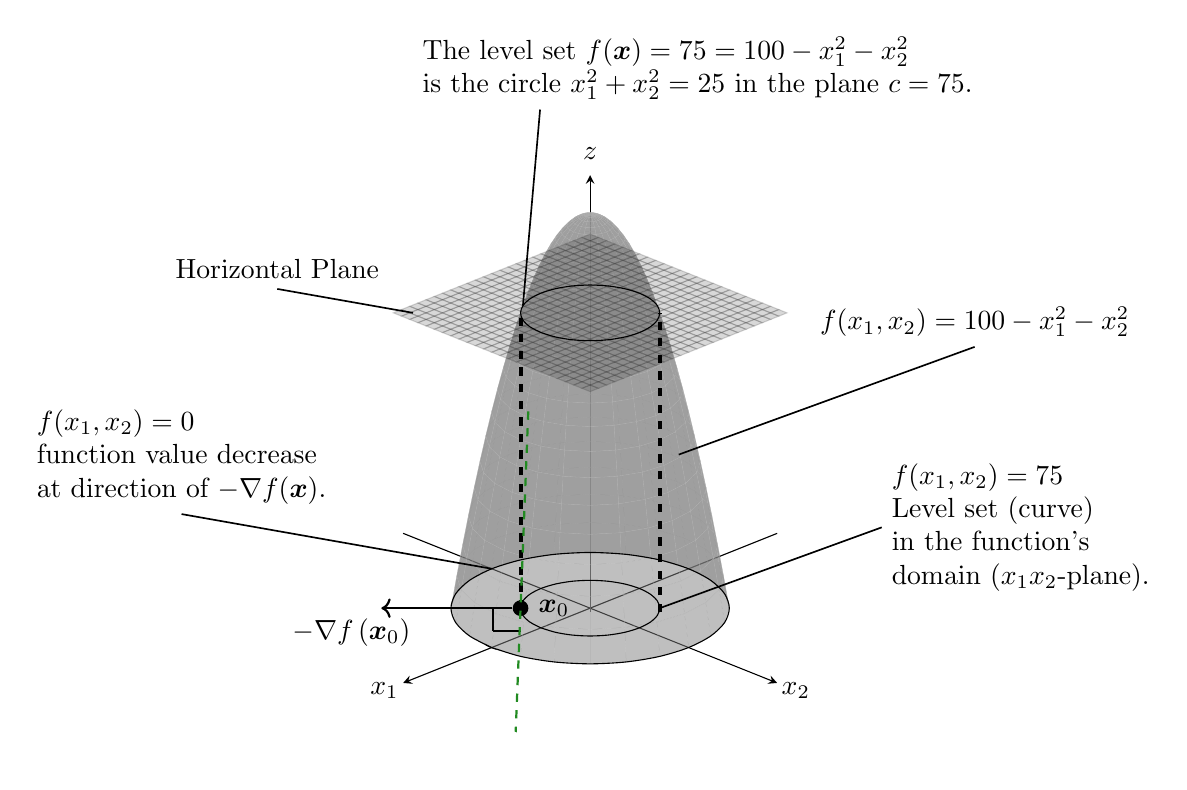
\begin{tikzpicture}
		\begin{axis}[
			view={110}{30}, % Adjust the viewing angle
			xlabel=\(x_1\), ylabel=\(x_2\), zlabel=\(z\), 
			xmin=-19, xmax=19,
			ymin=-19, ymax=19,
			zmin=-1, zmax=110,
			xtick=\empty, ytick=\empty, ztick=\empty,
			x={(-0.125cm,-0.05cm)}, y={(0.125cm,-0.05cm)}, z={(0cm,0.05cm)},
			axis lines=middle,
			every axis x label/.style={  at={(ticklabel* cs:1.05)},  },
			every axis y label/.style={  at={(ticklabel* cs:1.05)},  },
			every axis z label/.style={  at={(ticklabel* cs:1.05)},  },
			]
			
			% Paraboloid
			\addplot3[surf,
			shader=flat, draw=lightgray, fill=gray, ultra thin, 
			left color=gray, right color=gray, middle color=gray!25, 
			opacity=0.5, fill opacity=0.5,
			data cs=polar, domain=0:360, 
			y domain=0:10,
			restrict z to domain=0:101, 
			](x, y, 100-y^2);
			
			% Plane 
			\addplot3[surf, shader=faceted,
			colormap = {whiteblack}{color(0cm)  = (white);color(1cm) = (black)},
			% color=gray, 
			opacity=0.2, fill opacity=0.2, 
			domain=-10:10, 
			](x,y,75);
			
			% Circle at plane
			\addplot3[black, smooth, 
			domain=0:360, variable=\t
			]({5*cos(\t)},{5*sin(\t)},{75});
			
			% Circles at xy-plane
			\pgfplotsinvokeforeach{5, 10}{%%
				\pgfmathsetmacro\Radius{#1}
				\addplot3[black, smooth, 
				%no markers,
				%samples=55,% samples y=0, 
				domain=0:360, variable=\t
				]({\Radius*cos(\t)},{\Radius*sin(\t)},{0});
			}%%
			
			% Annotations 1/2
			\coordinate[label=](A) at ({5*cos(135)},{5*sin(45)},{0});
			\coordinate[label=](B) at (9, -9, 75);
			\coordinate[label=](C) at (-4, 5, 40);
			\coordinate[label=](D) at({5*cos(300)},{5*sin(300)},{75});
			\coordinate[label=](E) at (0,-10,0);
			
			% Draw dashed lines from surface to projection
			\draw[dashed, line width=0.5mm] (axis cs: {5*cos(45)},{5*sin(225)},0) -- (axis cs:{5*cos(45)},{5*sin(225)},75);
			\draw[dashed, line width=0.5mm] (axis cs: {5*cos(135)},{5*sin(45)},,0) -- (axis cs:{5*cos(135)},{5*sin(45)},75);
			
			% Point x0
			\node[label={right:\(\boldsymbol{x}_0\)},circle,fill,inner sep=2pt] (x0) at (axis cs:{5*cos(45)},{5*sin(225)},0) {};
			
			% Mark the intersection point x0 with an L-shape
			\draw[thick]  (axis cs:{7*cos(45)},{7*sin(225)},0) -- (axis cs:{7*cos(45)+2.9},{7*sin(225)+2.9},0);
			\draw[thick]  (axis cs:{7*cos(45)+2.9},{7*sin(225)+2.9},0) -- (axis cs:{5*cos(45)+2.9},{5*sin(225)+2.9},0);
			
			% Draw an approximate dashed tangent vector at x0
			\draw[dashed, thick, forestgreen] ($(x0)!-2.5cm!(7.2,0)$) -- ($(x0)!2.5cm!(7.2,0)$);
			
			% Draw the approximate gradient arrow
			\draw[thick, ->] (x0) --  (axis cs:{15*cos(45)},{15*sin(225)},0) node[at end, below left, xshift=0.5cm] {\(-\nabla f\left(\boldsymbol{x}_0\right)\)};
			
		\end{axis}
		
		
		% Annotations 2/2
		\draw[semithick] (A) -- +(20:3) node[right, align=left]{
			\(f(x_{1},x_{2})=75\)\\ Level set (curve) \\ in the function's \\ domain (\(x_{1}x_{2}\)-plane).};
		
		\draw[semithick] (B) -- +(170:1.75) node[above, align=left]{
			Horizontal Plane};
		
		\draw[semithick] (C) -- +(20:4) node[above]{\(f(x_{1},x_{2})=100-x_{1}^2-x_{2}^2\)};
		
		\draw[semithick] (D) -- +(85:2.5) node[above, align=left, xshift=2cm]{The level set  \( f(\boldsymbol{x}) = 75 = 100-x_{1}^2-x_{2}^2 \) \\ is the circle \(x_{1}^2+x_{2}^2=25\) in the plane \(c=75\).};
		
		\draw[semithick] (E) -- +(170:4) node[above, align=left]{
			\(f(x_{1},x_{2})=0\)\\ function value decrease \\ at direction of \(-\nabla f(\boldsymbol{x})\).};
		
	\end{tikzpicture}
\end{center}


\begin{itemize}

	\item \(\nabla f\left(\boldsymbol{x}_{0}\right)\) is the direction of \underline{maximum rate of increase} of \(f\) at \(\boldsymbol{x}_{0}\). 
	
	\item \(\nabla f\left(\boldsymbol{x}_{0}\right)\) is orthogonal to the level set through \(\boldsymbol{x}_{0}\) determined by \( f(\boldsymbol{x})=f\left(\boldsymbol{x}_{0}\right)\), 
	\[
	\nabla f\left(\boldsymbol{x}_0\right)^{\top}\left(\boldsymbol{x}-\boldsymbol{x}_0\right)=0 \quad \text { if } \quad \nabla f\left(\boldsymbol{x}_0\right) \neq 0.
	\]
	
	The direction of \textit{maximum rate of increase} of a real-valued differentiable function at a point is orthogonal to the level set of the function through that point.
	
	\item If \(\nabla f(\boldsymbol{x}) \neq 0\), \(- \dfrac{\nabla f(\boldsymbol{x})}{\|\nabla f(\boldsymbol{x})\|}\) is the direction of fastest decrease (\underline{steepest descent direction}) of \(f\) at \(\boldsymbol{x}\).

\end{itemize}


%------------------------------------------------------%
\subsection{Neighborhood}
\begin{itemize}
	\item A \underline{neighborhood} of a point \(x \in \mathbb{R}^n\) is defined by
	\[
	B_{\varepsilon}(\boldsymbol{x}):=\left\{\boldsymbol{y} \in \mathbb{R}^n:\|\boldsymbol{y}-\boldsymbol{x}\|<\varepsilon\right\}
	\]
	for some \(\varepsilon>0\). Note that \(B_{\varepsilon}(\boldsymbol{x})\) is open.

	\item Let \(S \subset \mathbb{R}^n\), then \(\boldsymbol{x}\) is called an \underline{interior point} of \(S\) if there exists \(\varepsilon>0\) such that \(B_{\varepsilon}(\boldsymbol{x}) \subset S\). The set of interior points of \(S\) is called the \underline{interior} of \(S\), denoted by \(\operatorname{int}(S)\).
	
	\item \(\boldsymbol{x}\) is called a \underline{boundary point} of \(S\) if any neighborhood of \(\boldsymbol{x}\) contains a point in \(S\) and a point in \(S^c\). A boundary point may or may not be in \(S\). The set of boundary points of \(S\) is called the \underline{boundary} of \(S\).
	
	\item A set \(S \subset \mathbb{R}^n\) is called \underline{open} if all its point are an interior points. \(S\) is called \underline{closed} if \(S^c\) is open.
	
	\item \(S\) is called \underline{bounded} if \(S \subset B_R(0)\) for some \(R>0 . S\) is called compact if \(S\) is \underline{closed} and bounded.
	
	\item Weierstrass theorem. Let \(S \subset \mathbb{R}^n\) be compact and \(f: S \rightarrow \mathbb{R}\) be continuous, then \(f\) attains maximum and minimum in \(S\).
	
	\item The intersection of finitely many half-spaces is called a \underline{polytope}. Note that a polytope is convex, since all half-spaces are convex.
	
	\item A nonempty bounded polytope is called a \underline{polyhedron}.
	
\end{itemize}



%------------------------------------------------------%
\subsection{Sequences and limits}

\begin{itemize}
	\item Let \(\boldsymbol{x}^{(1)}, \ldots, \boldsymbol{x}^{(k)}, \ldots\) be a sequence in \(\mathbb{R}^n\), then we say \(\boldsymbol{x}^{(k)}\) converges to \(\boldsymbol{x}^*\) if for any \(\varepsilon>0\), there exists \(K \in \mathbb{N}\) (depending on \(\varepsilon\) ) such that
	\[
	\left\|\boldsymbol{x}_k-\boldsymbol{x}^*\right\|<\varepsilon
	\]
	for all \(k \geq K\). This is denoted by \(\lim _{k \rightarrow \infty} \boldsymbol{x}^{(k)}=\boldsymbol{x}^*\) or \(\boldsymbol{x}^{(k)} \rightarrow \boldsymbol{x}^*\). \(\boldsymbol{x}^*\) is called the limit of the sequence \(\left(\boldsymbol{x}^{(k)}\right)_{k=1}^{\infty}\). If a sequence is convergent, then the limit is unique. Note that \(\boldsymbol{x}^{(k)} \rightarrow \boldsymbol{x}^*\) iff \(x_i^{(k)} \rightarrow x_i^*\) for all \(i=1, \ldots, n\).

	\item Theorem. A convergent sequence is bounded. A bounded sequence has at least one convergent subsequence.

	\item Theorem. A sequence \(\left(\boldsymbol{x}^{(k)}\right)_{k=1}^{\infty}\) converges to \(\boldsymbol{x}^*\) iff every subsequence of \(\left(\boldsymbol{x}^{(k)}\right)_{k=1}^{\infty}\) converges to \(\boldsymbol{x}^*\).
	
	\item We say \(f: \mathbb{R}^n \rightarrow \mathbb{R}^m\) is \underline{continuous} at \(\boldsymbol{x} \in \mathbb{R}^n\) if
	\[
	f\left(\boldsymbol{x}^{(k)}\right) \rightarrow f(\boldsymbol{x})
	\]
	for any sequence \(\boldsymbol{x}^{(k)} \rightarrow \boldsymbol{x}\).
	
	\item We say \(f\) is continuous on \(S \subset \mathbb{R}^n\) if \(f\) is continuous at every point of \(S\).
	
	\item Let \(f: \mathbb{R}^n \rightarrow \mathbb{R}\) and \(f \in \mathcal{C}^2\), and denote \(\boldsymbol{h}=\boldsymbol{b}-\boldsymbol{a}\), then
	\[
	f(\boldsymbol{b})=f(\boldsymbol{a})+D f(\boldsymbol{a}) \boldsymbol{h}+\frac{1}{2} \boldsymbol{h}^{\top} D^2 f(\boldsymbol{a}) \boldsymbol{h}+o\left(\|\boldsymbol{h}\|^2\right),
	\]
	where \(\lim _{\|\boldsymbol{h}\| \rightarrow 0} o\left(\|\boldsymbol{h}\|^2\right) /\|\boldsymbol{h}\|^2=0\).

\end{itemize}



\bigskip

\noindent
[Ref]: Edwin K.P. Chong, Stanislaw H. Żak, ``PART I MATHEMATICAL REVIEW" in ``\href{https://www.amazon.com/Introduction-Optimization-Edwin-K-Chong/dp/1118279018}{An introduction to optimization}", 4th Edition, John Wiley and Sons, Inc. 2013.



\end{document}
